\section{Menus and a Splash Screen: The Front End}

%\begin{itemize}
%    \item Lots of screenshots!
%    \item Explanation of menu system and splash screen, credits screen etc
%    \item Discussion of some UI principles used
%    \item mention sheen (GUI) framework from non-technical perspective (design / logic split etc).
%\end{itemize}

During the alpha stages of the development, the command line was the only way to specify whether a Serenity process should run as a client or a server, and what address and port to use, and so on. A significant part of the work in the beta stage (after Christmas) was to add the front end menus and UI. A whole framework was developed to build the menus, links between the different modes, and animate a splash screen. 

\begin{figure*}
	\hspace{-2.5em}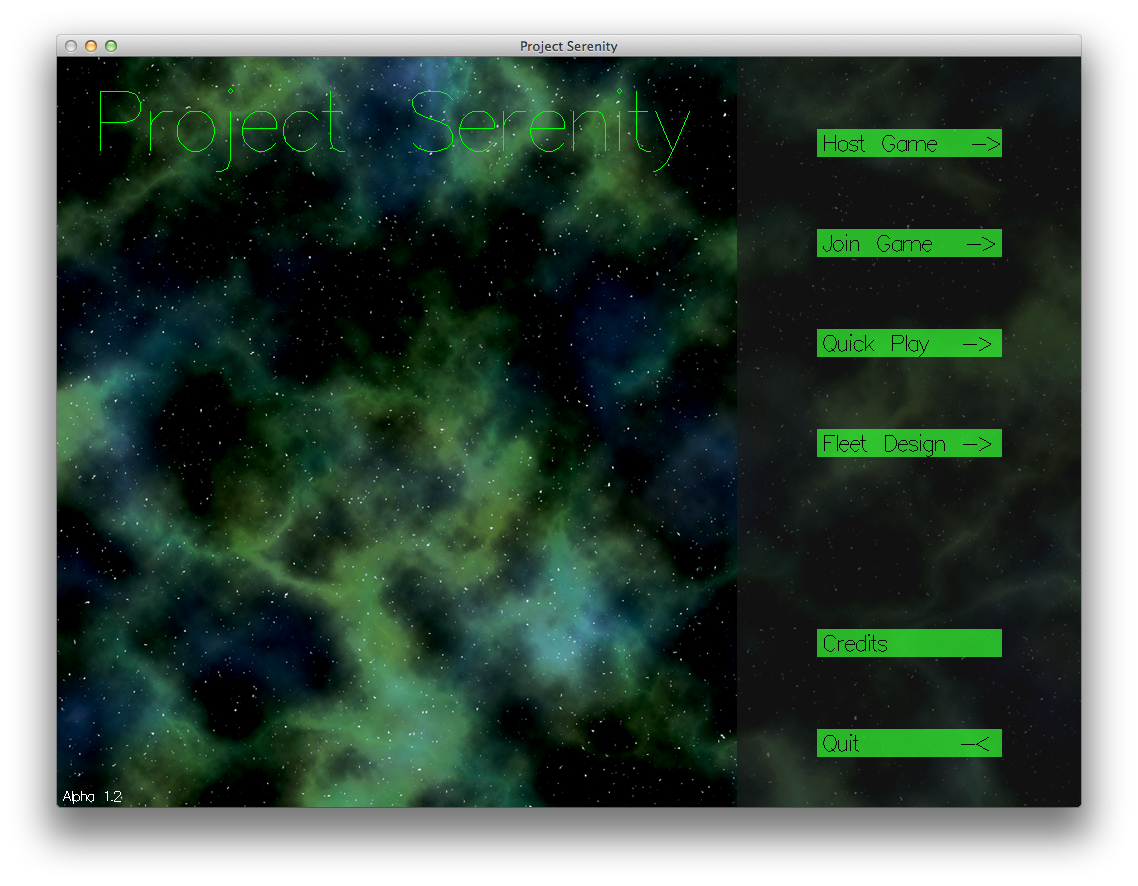
\includegraphics[width=17cm]{res/serenityscreens/01-mainmenu}
	\caption[Screenshot of the main menu]{Screenshot of the main menu.}
	\label{fig:mainmenu}
\end{figure*}

Figure~\ref{fig:mainmenu} shows the main menu design. The font is provided by Gloss, and while it is far from perfect it wasn't worth spending development time on improving it. The Splash screen animation was added mostly to help test the burgeoning framework, but it certainly adds a feeling of professionalism to the application. Two screenshots from the splash screen are shown in Figure~\ref{fig:splash}.

Considerable thought went into the design of the UI for hosting and joining a game. Controls enable and disable in a natural way that is clear in its method of use and no invalid state cannot be reached. These screens are shown in Figure~\ref{fig:hostjoin}.

\begin{figure*}[p]
	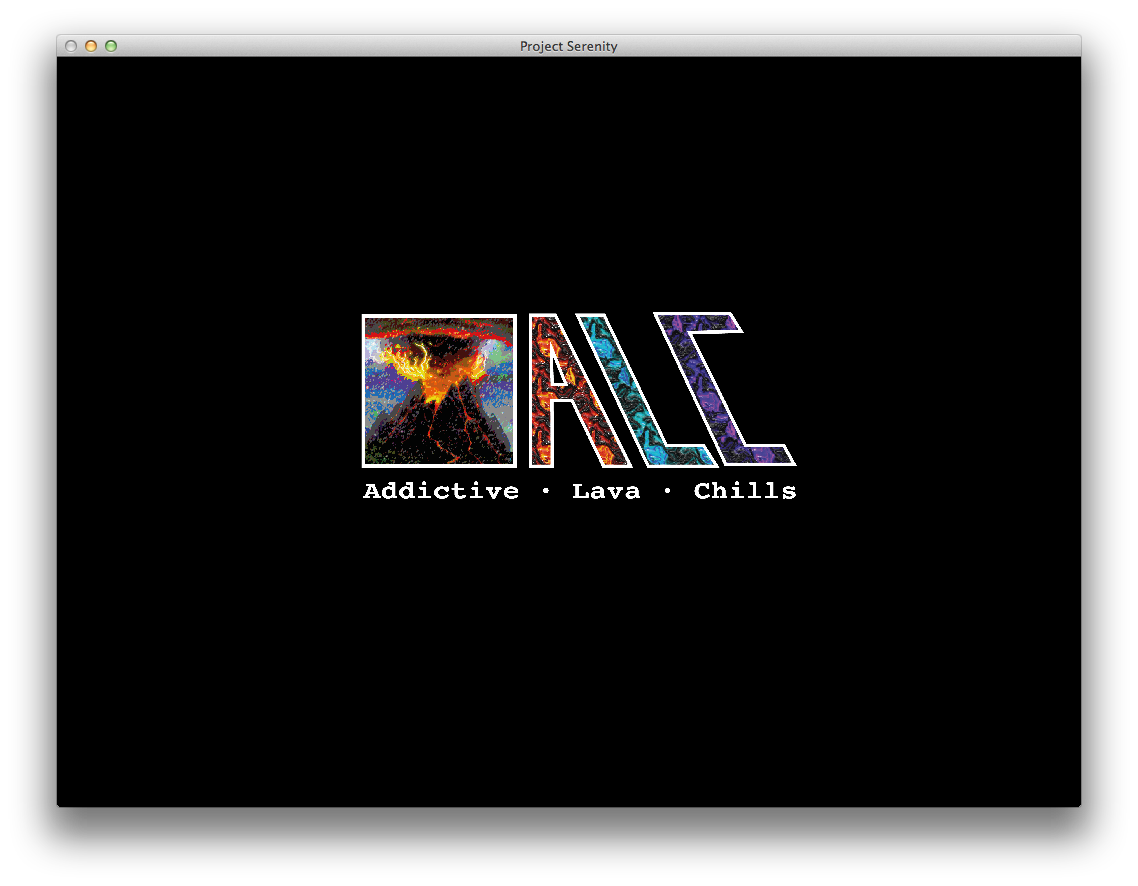
\includegraphics[width=15.5cm]{res/serenityscreens/07-splash1}
	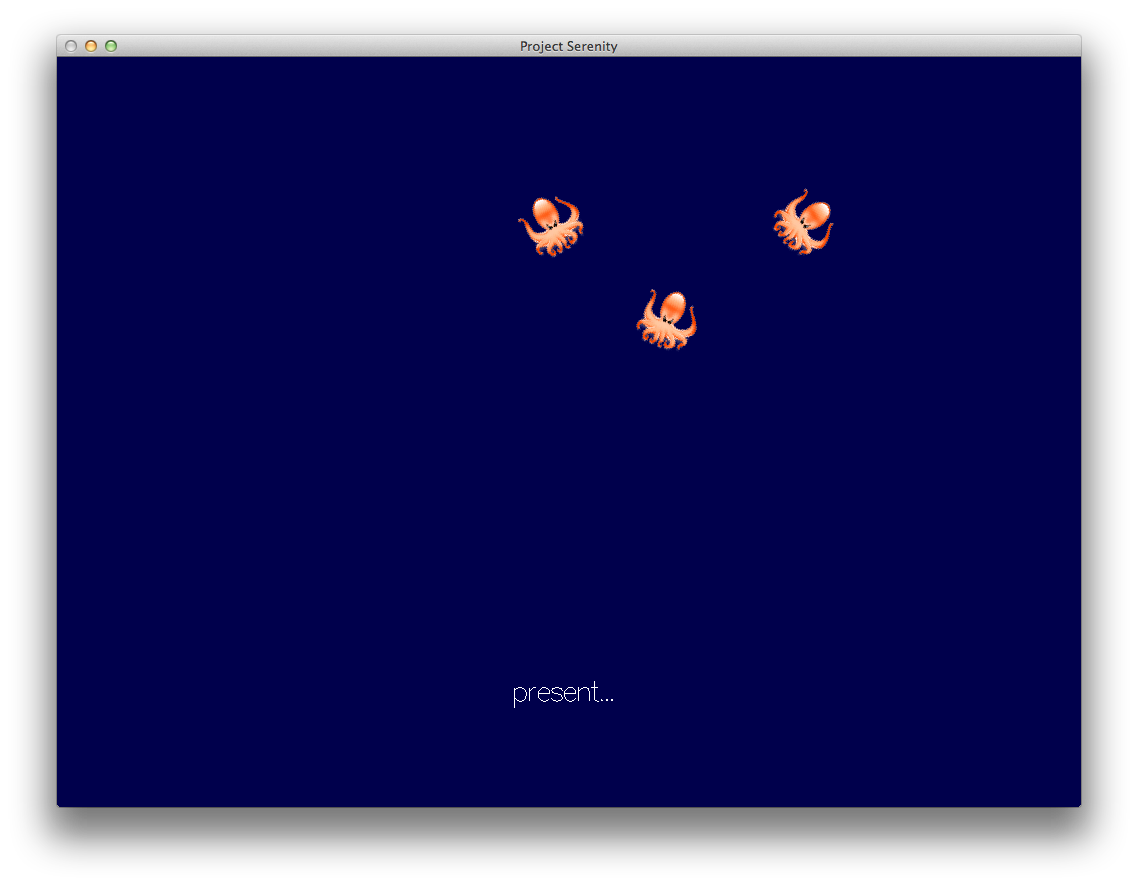
\includegraphics[width=15.5cm]{res/serenityscreens/08-splash2}
	\caption[Splash screens shown on launch]{Screenshot of the splash screens shown when the game is launched.}
	\label{fig:splash}
\end{figure*}

\begin{figure*}[p]
	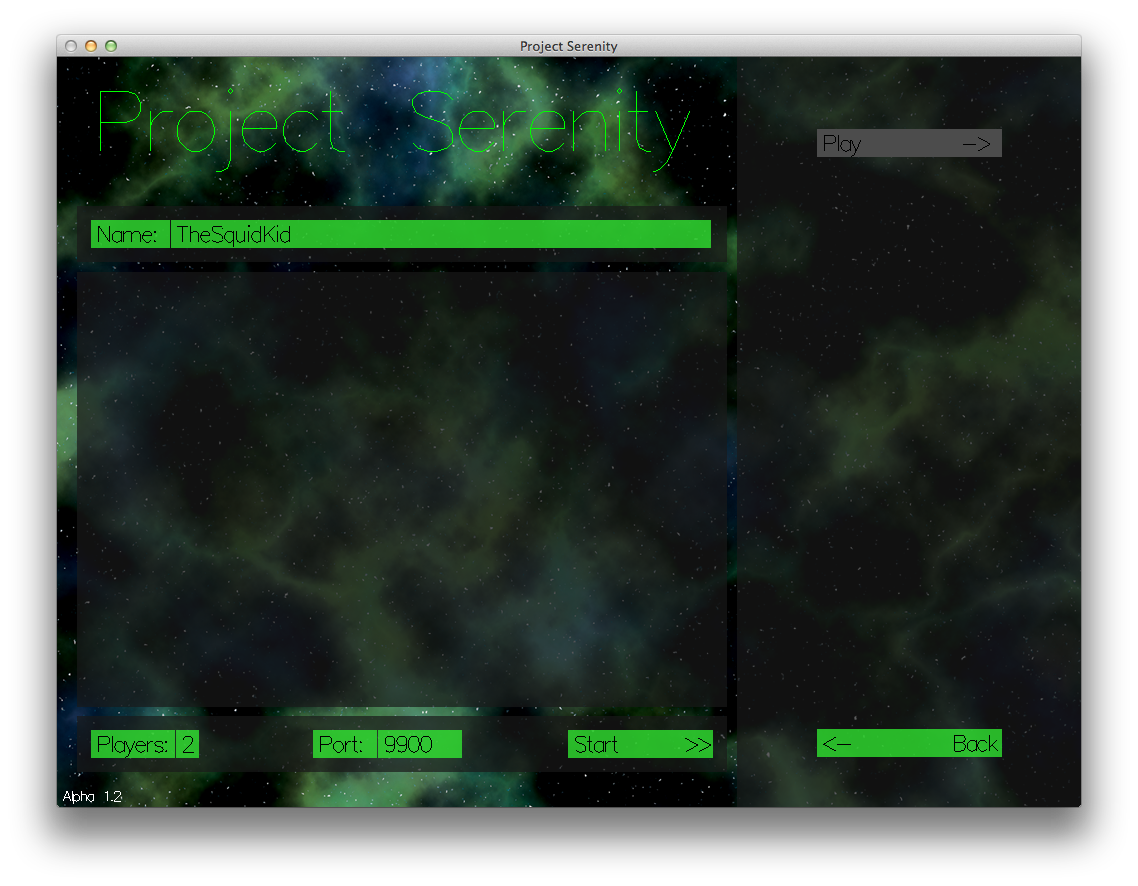
\includegraphics[width=15.5cm]{res/serenityscreens/02-host}
	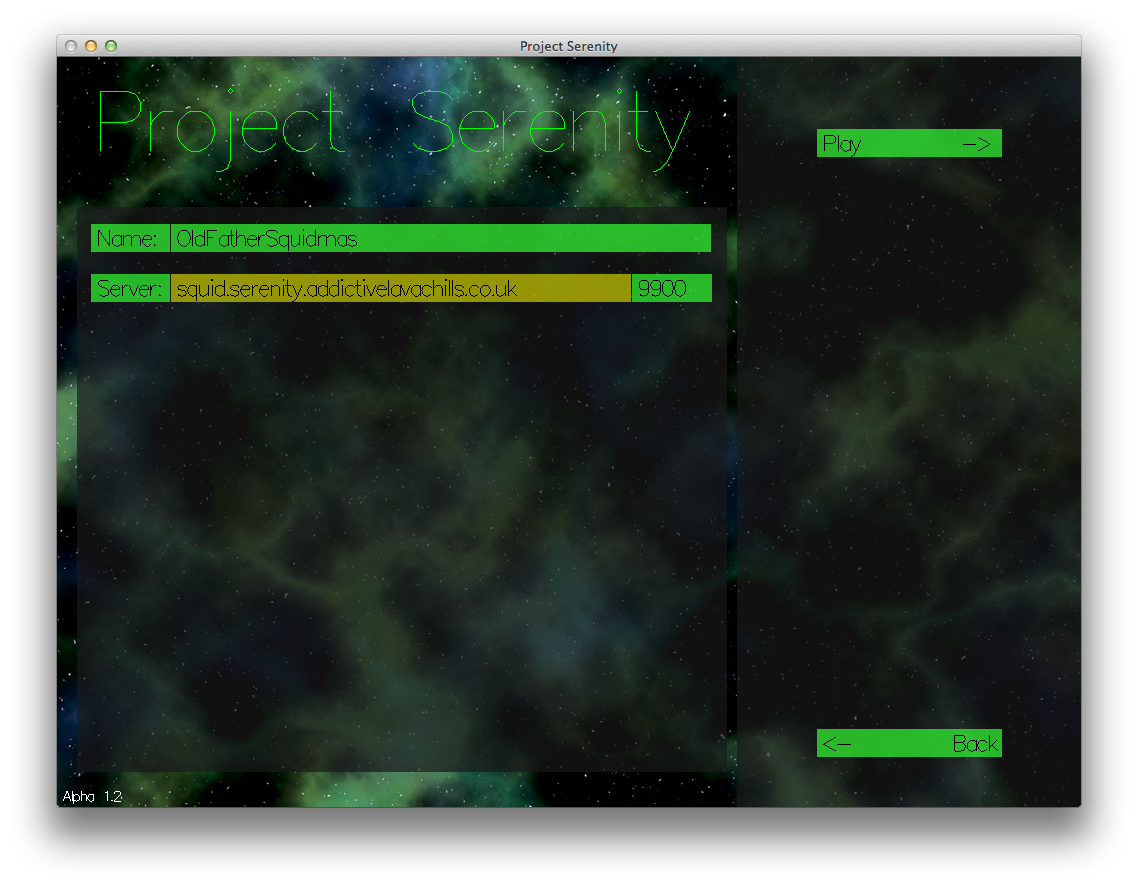
\includegraphics[width=15.5cm]{res/serenityscreens/03-join}
	\caption[Menus for hosting and joining battles]{Screenshot of the menus used to host and join battles.}
	\label{fig:hostjoin}
\end{figure*}

\begin{figure*}[t]
	\hspace{-2.5em}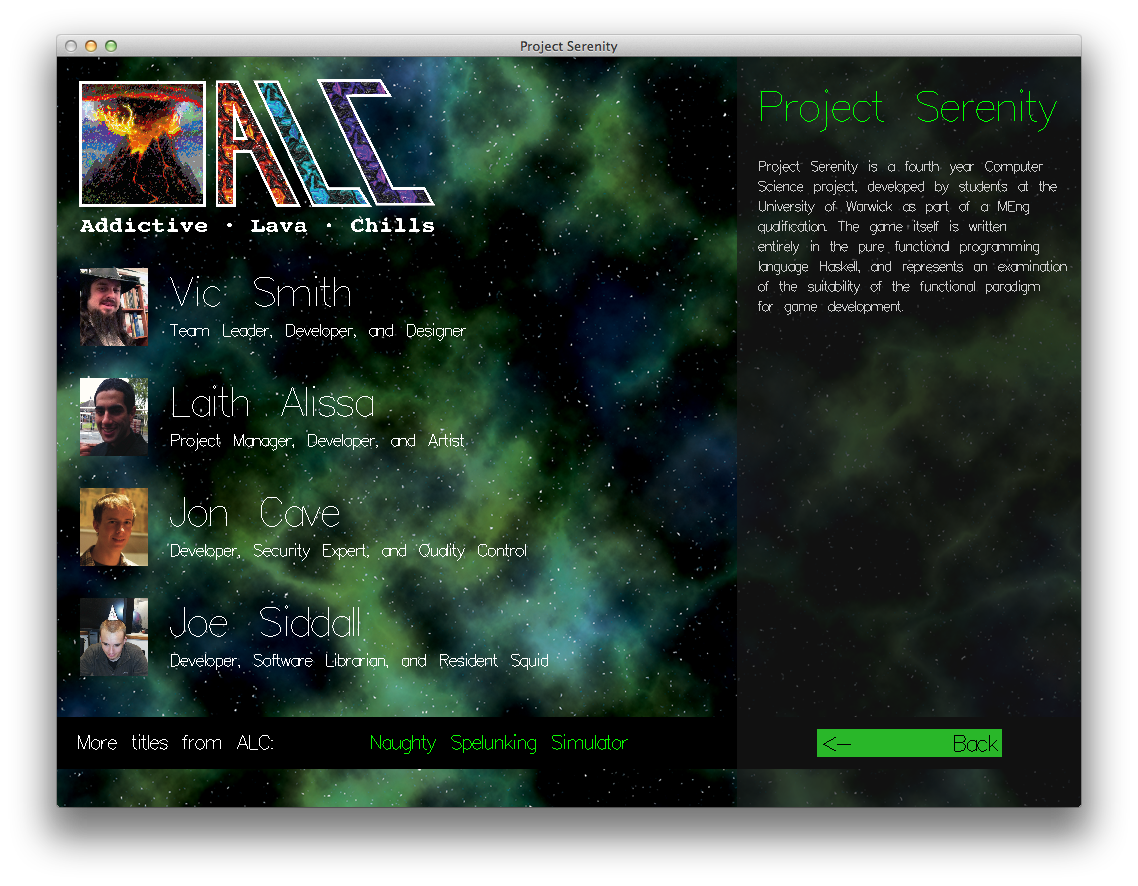
\includegraphics[width=17cm]{res/serenityscreens/05-credits}
	\caption[Screenshot of the credits screen]{Screenshot of the credits screen, showing the development team and the }
	\label{fig:credits}
\end{figure*}

A credits screen was also added to provide some information about the project and the developers. A random game name generator sneaked in as an easter egg. The credits screen is shown in Figure~\ref{fig:credits}.

The logo featured in the splash and credits screen is for the name given to the project group: \emph{Addictive Lava Chills} (formed from an anagram of the member's names). 
Both the green starscape used in the menus, and the layered nebula and stars used in the main game graphics were created from scratch using Guassian noise filters and cloud effects in Adobe\textregistered Photoshop.
